\section[تمرین اول - سوال اول: فشرده‌سازی تصویر با K-Means]{\faImage\ \ تمرین اول - سوال اول: فشرده‌سازی تصویر با الگوریتم K-Means}

\begin{stepbox}

\field{هدف و معرفی مسئله}{
هدف این تمرین، پیاده‌سازی الگوریتم \lr{K-Means Clustering} از ابتدا و استفاده از آن برای فشرده‌سازی تصاویر بود. در این روش، هر پیکسل تصویر به عنوان یک نمونه سه‌بعدی شامل مؤلفه‌های رنگی \lr{RGB} در نظر گرفته شده و با خوشه‌بندی این نمونه‌ها، تعداد رنگ‌های تصویر کاهش می‌یابد. در نهایت هر پیکسل با رنگ مرکز خوشه‌ی متناظر جایگزین می‌شود و تصویری با تعداد رنگ کمتر تولید خواهد شد.
}

\field{پیاده‌سازی الگوریتم K-Means}{
الگوریتم K-Means به صورت کامل و بدون استفاده از توابع آماده پیاده‌سازی شد. مراحل اجرای الگوریتم شامل موارد زیر است:

\begin{itemize}
\item محاسبه فاصله اقلیدسی هر نمونه تا تمامی مراکز خوشه
\item اختصاص هر نمونه به نزدیک‌ترین مرکز خوشه
\item محاسبه مجدد مراکز خوشه با استفاده از میانگین اعضای هر خوشه
\item تکرار مراحل فوق تا رسیدن به همگرایی یا پایان تعداد تکرارها
\end{itemize}

برای محاسبه فاصله بین نمونه‌ها و مراکز خوشه از فاصله اقلیدسی استفاده شد:

\[
d(x,c)=\sum_{i=1}^{n}(x_i-c_i)^2
\]

که در آن $x$ نمونه داده و $c$ مرکز خوشه است.
}

\field{اجرای الگوریتم روی مجموعه داده نمونه}{
در مرحله نخست، عملکرد الگوریتم روی مجموعه داده دوبعدی ارائه‌شده در تمرین بررسی شد. سه مرکز اولیه به صورت دستی انتخاب شدند و الگوریتم طی چند تکرار اجرا گردید. همان‌طور که در شکل مشاهده می‌شود، مراکز خوشه در هر تکرار به سمت میانگین داده‌های اختصاص یافته حرکت کرده و در نهایت به یک موقعیت پایدار همگرا شدند.

\vspace{0.4cm}

\begin{center}
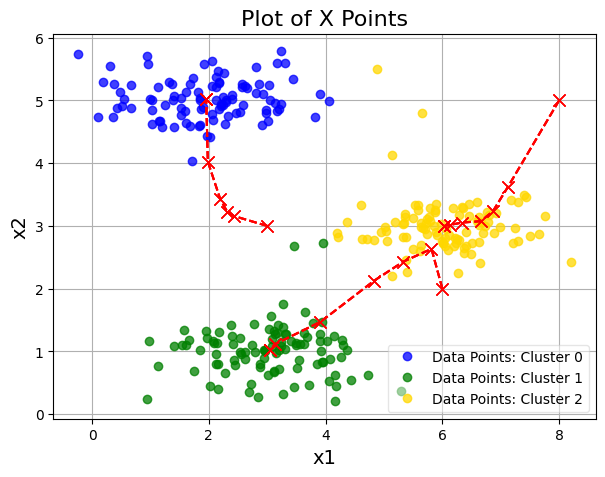
\includegraphics[width=.62\textwidth]{images/kmeans_dataset.png}
\captionof{figure}{همگرایی مراکز خوشه در اجرای الگوریتم K-Means}
\label{fig:kmeans_dataset}
\end{center}
}

\field{فشرده‌سازی تصویر}{
برای بررسی کاربرد عملی خوشه‌بندی، یک تصویر رنگی با ابعاد $128\times128$ انتخاب شد. ابتدا مقادیر رنگی تصویر به بازه $[0,1]$ نرمال شدند و سپس تصویر سه‌بعدی به ماتریسی با ابعاد

\[
16384 \times 3
\]

تبدیل گردید؛ به طوری که هر سطر نماینده یک پیکسل و هر ستون بیانگر یکی از مؤلفه‌های رنگی \lr{RGB} بود.

پس از آن، الگوریتم K-Means با تعداد خوشه

\[
K=16
\]

اجرا شد. در پایان، هر پیکسل با رنگ مرکز خوشه متناظر جایگزین شد و تصویر فشرده‌شده تولید گردید.
}

\field{نتایج و تحلیل}{
شکل زیر تصویر اصلی و تصویر فشرده‌شده را نشان می‌دهد. همان‌طور که مشاهده می‌شود، با وجود کاهش تعداد رنگ‌ها به تنها 16 رنگ، ساختار اصلی تصویر همچنان حفظ شده است و تنها بخشی از جزئیات رنگی از بین رفته‌اند.

\vspace{0.4cm}

\begin{center}
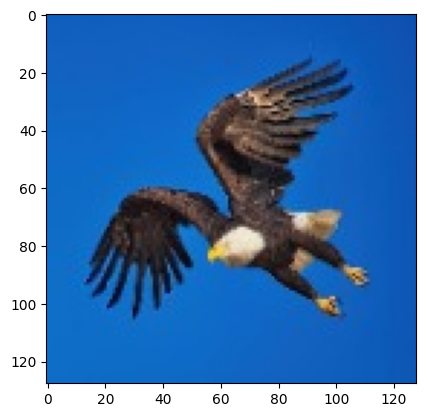
\includegraphics[width=.47\textwidth]{images/original_image.png}
\hfill
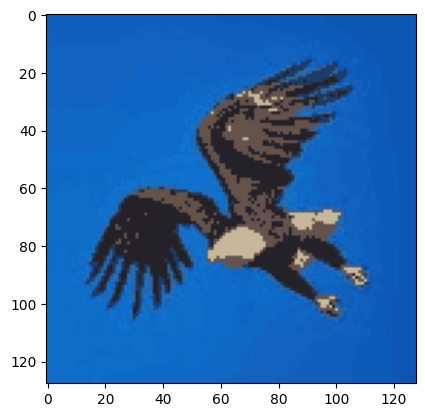
\includegraphics[width=.47\textwidth]{images/compressed_image.png}

\captionof{figure}{مقایسه تصویر اصلی و تصویر حاصل از فشرده‌سازی با الگوریتم K-Means}
\label{fig:compression}
\end{center}

کاهش تعداد رنگ‌ها باعث کاهش اطلاعات مورد نیاز برای ذخیره‌سازی تصویر می‌شود. هرچه مقدار $K$ افزایش یابد، کیفیت تصویر نهایی بیشتر خواهد شد؛ اما میزان فشرده‌سازی کاهش پیدا می‌کند. در مقابل، انتخاب مقادیر کوچک‌تر برای $K$ موجب کاهش بیشتر حجم داده‌ها خواهد شد اما افت کیفیت تصویر نیز محسوس‌تر خواهد بود.
}

\field{جمع‌بندی}{
در این تمرین، الگوریتم K-Means از پایه پیاده‌سازی و سپس در مسئله فشرده‌سازی تصویر به کار گرفته شد. نتایج نشان دادند که خوشه‌بندی رنگ‌ها می‌تواند بدون از بین رفتن ساختار کلی تصویر، تعداد رنگ‌های مورد استفاده را به طور قابل توجهی کاهش دهد. این آزمایش یکی از کاربردهای مهم الگوریتم‌های یادگیری بدون نظارت در پردازش تصویر را به خوبی نشان می‌دهد.
}

\end{stepbox}